\documentclass[9pt,twocolumn,twoside,lineno]{pnas-new}
% Use the lineno option to display guide line numbers if required.

\templatetype{pnasresearcharticle} % Choose template 
% {pnasresearcharticle} = Template for a two-column research article
% {pnasmathematics} %= Template for a one-column mathematics article
% {pnasinvited} %= Template for a PNAS invited submission

\title{Clique evolution of three brain networks via persistent homology}

% Use letters for affiliations, numbers to show equal authorship (if applicable) and to indicate the corresponding author
\author[a,1]{B. Ülgen Kılıç}

\affil[a]{University at Buffalo, Department of Mathematics}


% Please give the surname of the lead author for the running footer
\leadauthor{Kılıç} 

% Please add here a significance statement to explain the relevance of your work
\significancestatement{Human brain is one of the absolute unknowns of the modern times. Recent work has shown that by considering it as a network and focusing on the network properties might shed light on this mystery. Moreover, we can employ the machinery from mathematics and physics to understand the mechanisms driving this most advanced product of the natural selection as well as the origins of consciousness. }

% Please include corresponding author, author contribution and author declaration information
\correspondingauthor{\textsuperscript{2}To whom correspondence should be addressed. E-mail: bengieru@buffalo.edu}

% Keywords are not mandatory, but authors are strongly encouraged to provide them. If provided, please include two to five keywords, separated by the pipe symbol, e.g:
\keywords{Structural/Functional Brain network $|$ Human Connectome  $|$ Network neuroscience} 

\begin{abstract}
The network science has proven to be an exceptional tool for modeling and analyzing the real world systems in the past couple of decades. Among all the complex systems, the neural system has it's own unique corner in terms of it's self referencing nature due to the functional complexity of it. There is a caveat here by Godel, a famous mathematician, logician and philosopher, stating that it might not be possible to fully resolve the mysteries of a formal system for an observer inside of the system meaning that we are trying to understand the brain via our brain again. Is brain really that complex that it is able to understand it's own complexity? We don't know the answer yet, since we are far from understanding the all capabilities of the brain at the moment. However, this doesn't mean that we are not going to expand the frontiers as much as we can in neuroscience. With this motivation in mind, we want to combine the knowledge from a well-studied branch of mathematics, algebraic topology and persistent homology in particular is going to be the main tool we are employing. We start by comparing the evolution of the clique structures in a structural brain network with the resting state functional brain network.
\end{abstract}

\dates{This manuscript was compiled on \today}
\doi{\url{www.pnas.org/cgi/doi/10.1073/pnas.XXXXXXXXXX}}

\begin{document}

\maketitle
\thispagestyle{firststyle}
\ifthenelse{\boolean{shortarticle}}{\ifthenelse{\boolean{singlecolumn}}{\abscontentformatted}{\abscontent}}{}

% If your first paragraph (i.e. with the \dropcap) contains a list environment (quote, quotation, theorem, definition, enumerate, itemize...), the line after the list may have some extra indentation. If this is the case, add \parshape=0 to the end of the list environment.
\dropcap{I}t has been known that the human brain network has scale free topology, meaning that it's degree distribution is given by the controversial power law. Moreover, varying types of network measures, modularity, distribution of motif and hub structures can provide us meaningful information about the way this complex system works. One particular problem with the large brain networks is making associations between the structure and the function of the interactions between brain regions. In a large scale brain network, nodes are described by brain regions in the cortical and subcortical areas. In a structural brain network, the relations between the nodes are defined by white matter tracts which are obtained by BOLD signals. On the other hand, in a functional brain network, links are given by the magnitudes of functional correlations in activity. Thus, before making any sort of analysis, one should be cautious about the assumptions they are making because the way we analyze the brain via network science depends completely on the network that we want to choose since the nature of the connections are derived from different choices. For this to end, we are declaring the main purpose of this work is trying to reduce this ambiguity in network neuroscience, and compare these two types of networks in terms of lower connectivity regions which we elaborate more later and come up with a meaningful mapping if possible.

  In network theory, a k-clique is the subset of nodes in which every node is connected to k-1 others among the subset. A converse to this concept would be fully disconnected set of nodes. However, we are assuming our networks has one connected component. So, a partial converse can be defined as a hole, or a loop, in a network which can be thought of as removing some number of edges from the clique without changing the number of connected components. These regions in the brain networks can be characterized by a low connectivity region meaning that this part of the network does not completely shut down but works in a lower capacity, whereas a region without a hole, consisting of a clique is a stronger connectivity region in which every node of the network compounding the clique considered as engaging in the process of whatever the network does. It is shown that these lower connectivity regions might actually be responsible from resting-state dynamics, cognitive control and correlated network states(cite), so overlooking the activity of these regions may end up ignoring the potential research results.
  
\begin{figure}%[tbhp]
\centering
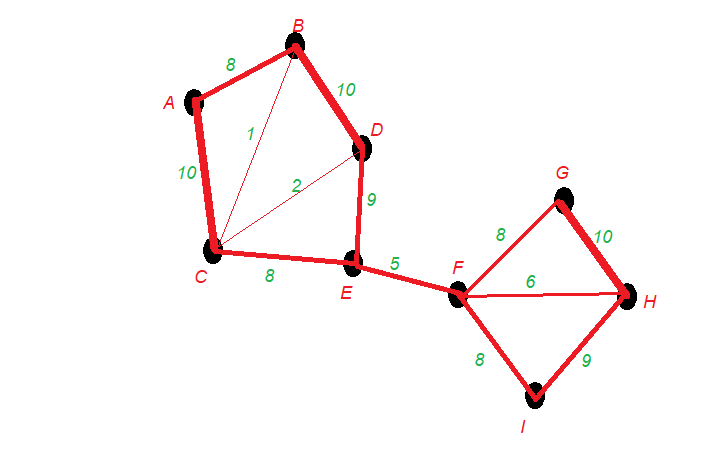
\includegraphics[width=.8\linewidth]{lower_connectivity.png}
\caption{An example of basic weighted network. The hole ABDEC is different from the hole FGHI in terms of depths. The former  loop appears when the all edges with weight 8 is present and dies the edge CD enters the filtration in total of depth 6. On the other hand, the loop FGHI appear at the same time as ABDEC but closes the edge FH enters the filtration at weight 6 in total of depth 2}
\label{fig:connectivty}
\end{figure}

Several attempts have been made to uncover this problem(cite) which are mostly rely on thresholding with respect to different scales... So, the problem with this approach is that thresholding value is decided by a user which most of the time ends up over looking the lower connectivity regions. In this work, we are employing a method which goes through every value of a range of finely divided thresholding values while keeping track of the information at each scale. 
\begin{figure*}%[tbhp]
\centering
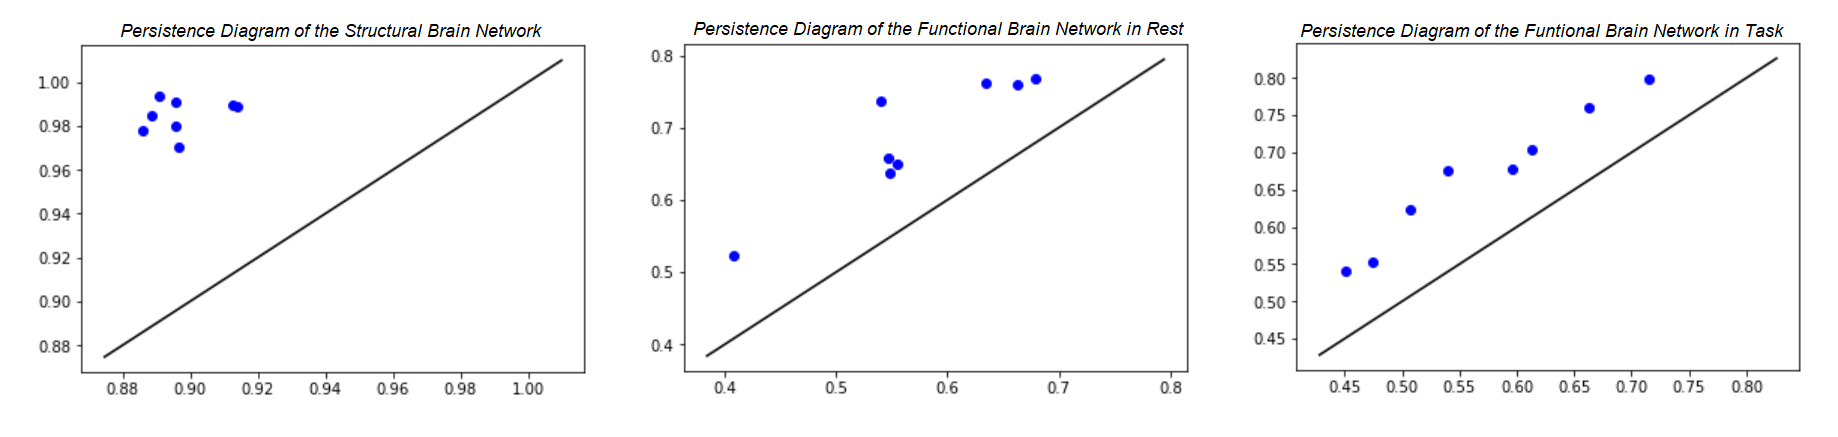
\includegraphics[width=18cm,height=6cm]{peristencediagrams.png}
\caption{Left: Strong edges compounding the loops in the structural brain network comes with strong edges making them a clique, so they don't appear in the persistence diagram. What we see is the weak edges, entering the filtration later on, whose filling edges are absent. Right: loops are appearing at every weight scale; weak edges lack of weaker edges making them a clique as well as strong edges lacking less strong edges making them a clique. Middle: the picture is sort of in the middle of the scale}
\end{figure*}

On the other hand, a loop in an abstract topological space can be characterized algebraically by the homology groups of that space. Given that a network can be constructed via combinatorial structures, so called simplices, every network can be given a topology i.e. every simple network is a topological object. Therefore, every network is prone to the tools of algebraic topology. So, just like degree, modularity or eigenvalue centrality, homology can be taught of as a network measure whose meaning is slightly less trivial. Yet, the meaning of a loop in the brain network setting is explained in the previous paragraph for reader to build bridges between two areas.

Persistent homology is a recent technique whose applications gained a lot of attention from different research fields over the past decade. Main idea of persistent homology is that building a nested sequence of subspaces, which is called a filtration, that approximates the original data set. Choosing how to build the filtration is like choosing the lenses that one looks at the data set(cite). Different filtration constructions would yield different results and most of the time filtration can be defined via a real valued function. More formally, let $X$ be the original data set we want to examine and $X_{0}\subset X_{1}\subset...\subset X_{N}=X $ be the filtration. Then, one can compute the homology of each individual spaces and keep track of the homological features that persisted in terms of filtration steps. The main assumption of the persistent homology is that actual signal in the data is going to persist for a long time whereas shorter persistent cycles are likely to be just noise.
In the brain network case, we indexed the filtration by the ranked edge weights in descending order. This will provide the edges with higher weight entering the filtration earlier and edges with lower edge weight later enabling the loop structures to be more significant before they get killed by a 2-cell, or a 3-clique. So, our construction goes as follows: given that we have a weighted network $N=(V,E,\omega)$, all 0-cells, the set of vertices $V$, are assumed to be having weight $0$, so they are going to be present in the space $X_{0}$. Then, in the first filtration step $X_{1}$, edges with maximum weight $\omega_{max}$ are going to enter the filtration. Then, in $X_{2}$, some edges with weight $\omega<\omega_{max}$ are entering the filtration so that $X_{1}\subset X_{2}$ and so on. Finally, the weight of a 2-cell is determined by minimum of it's coboundary so that at each step we'll have a closed 2-skeleton. Although, there are several packages in Python and MatLab that computes the persistent homology of a filtration, a good review article can be found (cite), we prefer to choose our own. This approach highlights not only the mesosopic regions of reduced connectivity but also how network properties evolve along the filtration.



\section*{Results}

We start with 14 individuals whose structural brain network is obtained via diffusion imaging and functional brain network in resting state is obtained via BOLD signals. For comparison, we also measure the BOLD signals in a modular arithmetic test and turned it into a functional brain network. Then, we averaged the data among 14 individuals and carry on the analysis with only three networks: structural, functional in rest and functional in task. After the computation of 1st homology generators of each networks, we kept the 8 cycles that persisted most in each of them. Figure 1 shows the persistence diagrams corresponding to each instance. The appearance of the lower connectivity regions throughout the filtration is different in each case. Even though we didn't realize a significant difference in terms of persistence durations of these cycles, in the structural network, we noticed all 8 generators born towards the end of the filtration whereas functional brain network in rest shows a little more linear distribution throughout the filtration. Functional brain network in task demonstrates the most linear distribution meaning that the brain turns into a more organized state during a task engaging different levels of lower connectivity regions i.e. several loops born at different weights with pretty much the same depth. On the other hand, in the structural brain network, holes are tend to born and die around the same weight scale. 

\subsection*{Author Affiliations}

Include department, institution, and complete address, with the ZIP/postal code, for each author. Use lower case letters to match authors with institutions, as shown in the example. Authors with an ORCID ID may supply this information at submission.

\subsection*{Submitting Manuscripts}

All authors must submit their articles at \href{http://www.pnascentral.org/cgi-bin/main.plex}{PNAScentral}. If you are using Overleaf to write your article, you can use the ``Submit to PNAS'' option in the top bar of the editor window. 

\subsection*{Format}

Many authors find it useful to organize their manuscripts with the following order of sections;  Title, Author Affiliation, Keywords, Abstract, Significance Statement, Results, Discussion, Materials and methods, Acknowledgments, and References. Other orders and headings are permitted.

\subsection*{Manuscript Length}

PNAS generally uses a two-column format averaging 67 characters, including spaces, per line. The maximum length of a Direct Submission research article is six pages and a Direct Submission Plus research article is ten pages including all text, spaces, and the number of characters displaced by figures, tables, and equations.  When submitting tables, figures, and/or equations in addition to text, keep the text for your manuscript under 39,000 characters (including spaces) for Direct Submissions and 72,000 characters (including spaces) for Direct Submission Plus.

\subsection*{References}

References should be cited in numerical order as they appear in text; this will be done automatically via bibtex, e.g. \cite{belkin2002using} and \cite{berard1994embedding,coifman2005geometric}. All references should be included in the main manuscript file.  

\subsection*{Data Archival}

PNAS must be able to archive the data essential to a published article. Where such archiving is not possible, deposition of data in public databases, such as GenBank, ArrayExpress, Protein Data Bank, Unidata, and others outlined in the Information for Authors, is acceptable.

\subsection*{Language-Editing Services}
Prior to submission, authors who believe their manuscripts would benefit from professional editing are encouraged to use a language-editing service (see list at www.pnas.org/site/authors/language-editing.xhtml). PNAS does not take responsibility for or endorse these services, and their use has no bearing on acceptance of a manuscript for publication. 

\begin{figure}%[tbhp]
\centering

\includegraphics[width=.8\linewidth]{frog.eps}
\caption{Placeholder image of a frog with a long example caption to show justification setting.}
\label{fig:frog}
\end{figure}


\begin{SCfigure*}[\sidecaptionrelwidth][t]
\centering
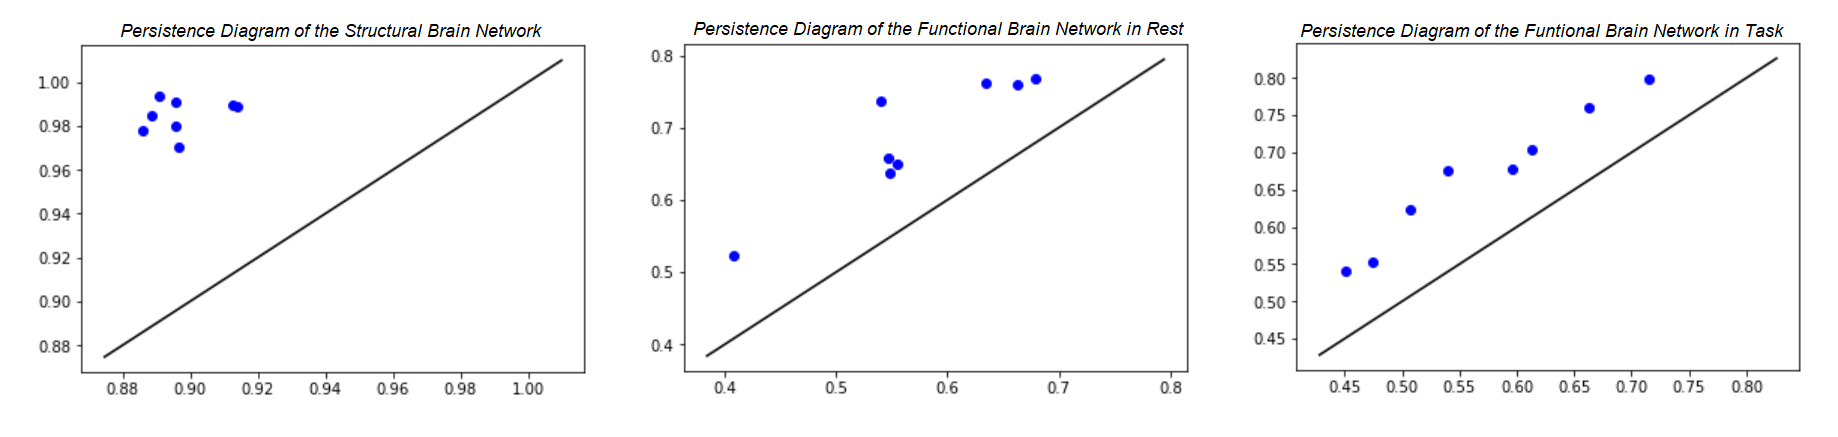
\includegraphics[width=18cm,height=6cm]{peristencediagrams.png}
\caption{This caption would be placed at the side of the figure, rather than below it.}
\end{SCfigure*}

\subsection*{Digital Figures}

Only TIFF, EPS, and high-resolution PDF for Mac or PC are allowed for figures that will appear in the main text, and images must be final size. Authors may submit U3D or PRC files for 3D images; these must be accompanied by 2D representations in TIFF, EPS, or high-resolution PDF format.  Color images must be in RGB (red, green, blue) mode. Include the font files for any text. 

Figures and Tables should be labelled and referenced in the standard way using the \verb|\label{}| and \verb|\ref{}| commands.

Figure \ref{fig:frog} shows an example of how to insert a column-wide figure. To insert a figure wider than one column, please use the \verb|\begin{figure*}...\end{figure*}| environment. Figures wider than one column should be sized to 11.4 cm or 17.8 cm wide. Use \verb|\begin{SCfigure*}...\end{SCfigure*}| for a wide figure with side captions.

\subsection*{Tables}
In addition to including your tables within this manuscript file, PNAS requires that each table be uploaded to the submission separately as a “Table” file.  Please ensure that each table .tex file contains a preamble, the \verb|\begin{document}| command, and the \verb|\end{document}| command. This is necessary so that the submission system can convert each file to PDF.

\subsection*{Single column equations}

Authors may use 1- or 2-column equations in their article, according to their preference.

To allow an equation to span both columns, use the \verb|\begin{figure*}...\end{figure*}| environment mentioned above for figures.

Note that the use of the \verb|widetext| environment for equations is not recommended, and should not be used. 

\begin{figure*}[bt!]
\begin{align*}
(x+y)^3&=(x+y)(x+y)^2\\
       &=(x+y)(x^2+2xy+y^2) \numberthis \label{eqn:example} \\
       &=x^3+3x^2y+3xy^3+x^3. 
\end{align*}
\end{figure*}


\begin{table}%[tbhp]
\centering
\caption{Comparison of the fitted potential energy surfaces and ab initio benchmark electronic energy calculations}
\begin{tabular}{lrrr}
Species & CBS & CV & G3 \\
\midrule
1. Acetaldehyde & 0.0 & 0.0 & 0.0 \\
2. Vinyl alcohol & 9.1 & 9.6 & 13.5 \\
3. Hydroxyethylidene & 50.8 & 51.2 & 54.0\\
\bottomrule
\end{tabular}

\addtabletext{nomenclature for the TSs refers to the numbered species in the table.}
\end{table}

\subsection*{Supporting Information (SI)}

Authors should submit SI as a single separate PDF file, combining all text, figures, tables, movie legends, and SI references.  PNAS will publish SI uncomposed, as the authors have provided it.  Additional details can be found here: \href{http://www.pnas.org/page/authors/journal-policies}{policy on SI}.  For SI formatting instructions click \href{https://www.pnascentral.org/cgi-bin/main.plex?form_type=display_auth_si_instructions}{here}.  The PNAS Overleaf SI template can be found \href{https://www.overleaf.com/latex/templates/pnas-template-for-supplementary-information/wqfsfqwyjtsd}{here}.  Refer to the SI Appendix in the manuscript at an appropriate point in the text. Number supporting figures and tables starting with S1, S2, etc.

Authors who place detailed materials and methods in an SI Appendix must provide sufficient detail in the main text methods to enable a reader to follow the logic of the procedures and results and also must reference the SI methods. If a paper is fundamentally a study of a new method or technique, then the methods must be described completely in the main text.

\subsubsection*{SI Datasets} 

Supply Excel (.xls), RTF, or PDF files. This file type will be published in raw format and will not be edited or composed.


\subsubsection*{SI Movies}

Supply Audio Video Interleave (avi), Quicktime (mov), Windows Media (wmv), animated GIF (gif), or MPEG files and submit a brief legend for each movie in a Word or RTF file. All movies should be submitted at the desired reproduction size and length. Movies should be no more than 10 MB in size.


\subsubsection*{3D Figures}

Supply a composable U3D or PRC file so that it may be edited and composed. Authors may submit a PDF file but please note it will be published in raw format and will not be edited or composed.


\matmethods{Please describe your materials and methods here. This can be more than one paragraph, and may contain subsections and equations as required. Authors should include a statement in the methods section describing how readers will be able to access the data in the paper. 

\subsection*{Subsection for Method}
Example text for subsection.
}

\showmatmethods{} % Display the Materials and Methods section

\acknow{Please include your acknowledgments here, set in a single paragraph. Please do not include any acknowledgments in the Supporting Information, or anywhere else in the manuscript.}

\showacknow{} % Display the acknowledgments section

% Bibliography
\bibliography{pnas-sample}

\end{document}